% !TeX spellcheck = <none>
\setcounter{page}{1}
\clubpenalty=100000  % Недопуск Висячей строки в начале страницы
\widowpenalty=100000 %Недопуск висячей строки в конце абзаца
%%%%%%%%%%%%%%%%%%%%%%%%%%%%%%%%%%%%%%%%
%      Шапка экспертной организации  
%%%%%%%%%%%%%%%%%%%%%%%%%%%%%%%%%%%%%%%%
%%%%%%%%%%%%%%%%%%%%%%%%%%%%%%%%%%%%%%%%%
%
%   Экспертная организация ООО Южнорегиональная экспертная группа
%
%%%%%%%%%%%%%%%%%%%%%%%%%%%%%%%%%%%%%%%%%
\noindent %\qrcode[height=21mm]{\NomerDoc от \окончено }  %%% Добавлен QR-Code
\begin{pspicture}(21mm,21mm)
\obeylines
\psbarcode{%
%	\NomerDoc от \окончено
	BEGIN:VCARD^^J
	VERSION:4.0^^J
	%N:Мраморнов; Александр; Вчеславович^^J
	FN:Александр Мраморнов^^J
%	ORG:IP Alexandr Mramornov^^J
	TITLE: эксперт
	ORG: ИП
	URL:http://www.yourexp.ru^^J
	EMAIL:4516611@gmail.com^^J
	TEL:+7-918-451-6611^^J
	ADR:г. Краснодар, с/т № 2 А/О «Югтекс», ул. Зеленая, 472^^J
	END:VCARD
}{width=1.0 height=1.0}{qrcode}%
\end{pspicture}%%% Добавлен QR-Code
\vspace{-4mm}
\begin{center}
	\large\textbf{ИНДИВИДУАЛЬНЫЙ\quad ПРЕДПРИНИМАТЕЛЬ  \\[-1.5mm] МРАМОРНОВ  АЛЕКСАНДР ВЯЧЕСЛАВОВИЧ \\[-5.5mm]}
	%  
	\noindent\rule{\textwidth}{2pt}\\[-6mm]  % Горизонтальная линия
	% \line(1,0){460}% (1,0) -горизонтальная линия, и (0,1) - вертикальная 
\end{center}

\begin{center}
	\begin{footnotesize}\setstretch{0.3}
		%	\small\textbf\setlength   	%\raisebox{5mm}
		\vspace{-3.5mm}г. Краснодар, с/т № 2 А/О «Югтекс», ул. Зеленая, 472, 
		Телефон: 8-918-451-66-11, e-mail: 4516611@gmail.com\\ [-2mm]{ИНН\quad 231200665168\quad ОГРНИП \quad 310231220400043}
	\end{footnotesize}	\\[10mm]
\end{center}


\begin{flushright}
% 
	 \hfill	Краснодар, 2020    \\[8mm]
\end{flushright}
\begin{center}
	\LARGE\textbf{ЭКСПЕРТНОЕ ЗАКЛЮЧЕНИЕ}
	\bigskip\\[0mm]
	%	{\normnumxtbf{\NomerDoc}}	}{den}
\end{center}
\par
\vspace{-6mm}
\noindent независимой технической экспертизы по определению размера расходов на восстановительный ремонт транспортного средства   \тс  \\[2mm]

%\raggedright 
%\def\hrf#1{\hbox to#1{\hrulefill}}
\noindent \textbf{№ \NomerDoc}\hfill           \textbf{\окончено}\\%[2mm]
%Приостановлено\hfill      \datastop\\
%Возобновлено\hfill          \datarestart\\
%Окончено\hfill                \dataend\\%[4mm]

\noindent\parbox[l][16mm]{16.5cm}
{\def\hrf#1{\hbox to#1{\hrulefill}}
	\noindent Начато\hfill            \datastart\\%[2mm]
	%	Приостановлено\hfill      \datastop\\
	%	Возобновлено\hfill          \datarestart\\
	Окончено\hfill                \окончено
}
\relax

%%%%%%%%%%%% Если судебка
%
%\datastart г. ~в {\small ООО~ "ЮЖНО-РЕГИОНАЛЬНАЯ ЭКСПЕРТНАЯ ГРУППА"} \,  при определении  \, \sud  \,  от \, \dataopr \, о назначении \opr \, по гражданскому делу \delonum \, поступили:
%
%\begin{enumerate}\setlist{nolistsep}\item  Материалы гражданского дела \delonum \, в двух томах, том 1 на 276 листах, том 2  на 143 листах.\\[-2mm]
%	%	\item  
%\end{enumerate}
%
%%%%%%%%%%%%  Если независимая
\vspace{4mm}
Составлено на основании	договора № \NomerDoc\,  на оказание услуг по проведению независимой технической экспертизы (далее экспертиза)  транспортного средства и письменного заявления заказчика о проведении экспертизы.

Заказчик  экспертизы: \заказчик, \адресзаказчика. 

Полис ОСАГО: \polis.

% Документ, удостоверяющий личность заказчика: водительское удостоверение    03\ 16\ 422344\ выдан 09.06.2011

%Транспортное средство виновника ДТП:  не предоставлялось.

\paragraph*{}
Экспертиза произведена  экспертом--техником
%{\small ООО "ЮЖНО-РЕГИОНАЛЬНАЯ ЭКСПЕРТНАЯ ГРУППА"}
\,  Мраморновым Александром Вячеславовичем, имеющим высшее  образование по специальности «техническая физика», диплом РВ № 311964 от 28.02.1989, квалификация -- инженер-физик, специальное образование в области оценки: Диплом ПП-1 № 037211 Российской экономической академии им. Г.В. Плеханова, квалификация -- оценка и экспертиза объектов и прав собственности, специальное образование в области независимой технической экспертизы транспортных средств: Диплом ПП-I № 424167, квалификация: эксперт-техник (специализация 150210 специальности 190601.65 – Автомобили и автомобильное хозяйство), состоящий в Государственном реестре экспертов-техников (№ в реестре 256, https://data.gov.ru/opendata/7707211418-experts,  общий трудовой  стаж 29 лет, стаж  экспертной работы  12 лет. \par Заключение подготовлено по месту фактического расположения ИП по адресу: г. Краснодар, с/т № 2 А/О «Югтекс», ул. Зелёная, 472.
  % Шапка организации ИП
%%%%%%%%%%%%%%%%%%%%%%%%%%%%%%%%%%%%%%%%%%
%
%   Экспертная организация ООО Южнорегиональная экспертная группа
%
%%%%%%%%%%%%%%%%%%%%%%%%%%%%%%%%%%%%%%%%%
\noindent %\qrcode[height=21mm]{\NomerDoc от \окончено }  %%% Добавлен QR-Code
\begin{pspicture}(21mm,21mm)
\obeylines
\psbarcode{%
	%\NomerDoc от \окончено
	BEGIN:VCARD^^J
	VERSION:4.0^^J
	%N:Мраморнов; Александр; Вчеславович^^J
	FN:Александр Мраморнов^^J
%	ORG:IP Alexandr Mramornov^^J
	TITLE: эксперт
	ORG: ИП
	URL:http://www.yourexp.ru^^J
	EMAIL:4516611@gmail.com^^J
	TEL:+7-918-451-6611^^J
	ADR:г. Краснодар, с/т № 2 А/О «Югтекс», ул. Зеленая, 472^^J
	END:VCARD
}{width=1.0 height=1.0}{qrcode}%
\end{pspicture}
\begin{center}
	\normalsize\textbf{$\cdots$\\[-1.5mm] <<$\cdots$>> \\[-5mm]}
	%  
	\noindent\rule{\textwidth}{1pt}\\[-6mm]  % Горизонтальная линия
	% \line(1,0){460}% (1,0) -горизонтальная линия, и (0,1) - вертикальная 
\end{center}

\begin{center}
	\begin{footnotesize}\setstretch{0.3}
		%	\small\textbf\setlength   	%\raisebox{5mm}
		\vspace{-3.5mm}$\cdots$\\[0mm]
		Телефон: \quad $\cdots$, e-mail:\quad $\cdots$\\ [-2mm]{$\cdots$\quad$\cdots$}
	\end{footnotesize}	\\[10mm]
\end{center}


\begin{flushright}
	%Краснодар,
	$\cdots$, 2020    \\[8mm]
\end{flushright}
\begin{center}
	\LARGE\textbf{ ЗАКЛЮЧЕНИЕ ЭКСПЕРТА}
	\bigskip\\[0mm]
	%	{\normnumxtbf{\NomerDoc}}	}{den}
\end{center}
\par
\vspace{-3mm}\noindent по гражданскому делу \delonum \, по иску \isk \\[0mm]

%\raggedright 
%\def\hrf#1{\hbox to#1{\hrulefill}}
\noindent \textbf{№ $\cdots$}\hfill           \textbf{\окончено}\\%[2mm]
%Приостановлено\hfill      \datastop\\
%Возобновлено\hfill          \datarestart\\
%Окончено\hfill                \dataend\\%[4mm]

\noindent\parbox[l][16mm]{16.5cm}
{\def\hrf#1{\hbox to#1{\hrulefill}}
	\noindent Начато\hfill            \datastart\\%[2mm]
	%	Приостановлено\hfill      \datastop\\
	%	Возобновлено\hfill          \datarestart\\
	Окончено\hfill                \окончено\\%[4mm]
}
\relax

\datastart г. ~в {\small $\cdots$} \,  при определении  \, \sud  \,  от \, \dataopr \, о назначении \opr \, по гражданскому делу \delonum \, поступили:

\begin{enumerate}\setlist{nolistsep}\item  Материалы гражданского дела \delonum \\[-2mm]
	%	\item  
\end{enumerate}Экспертиза произведена экспертом  $\cdots$  % Шапка организации ИП

Экспертное заключение составлено на основании	договора № \NomerDoc\,  возмездного оказания услуг по проведению независимой технической экспертизы (далее экспертиза)  транспортного средства и письменного заявления заказчика о проведении экспертизы.

Заказчик  экспертизы: \заказчик, \адресзаказчика. 

Полис ОСАГО: \polis.

% Документ, удостоверяющий личность заказчика: водительское удостоверение    03\ 16\ 422344\ выдан 09.06.2011

%Транспортное средство виновника ДТП:  не предоставлялось.

\paragraph*{}
  Производство исследования выполнено экспертом   Юрковой Еленой Александровной, имеющей высшее образование по специальности «Городской кадастр» с присвоением квалификации «Инженер». Специальное образование в области технической экспертизы транспортных средств: диплом о профессиональной переподготовке № 232402948332 Рег.№ 2009-ЭТ от 30.11.2015 г. по программе «Программа профессиональной переподготовки экспертов-техников» -  «Независимая техническая экспертиза транспортных средств». Состоит в государственном реестре экспертов-техников, осуществляющих независимую техническую экспертизу транспортных средств, регистрационный №5273 (протокол от 11.02.2016г. №. 1)  Специальное образование в области оценки: диплом о профессиональной переподготовке ПП-1 № 052044 от 11.06.2008 года  по программе «Оценка стоимости предприятия (бизнеса)» выдан ГОУ ВПО «Кубанский Государственный Технологический Университет». Квалификационный аттестат в области оценочной деятельности №006138-2 от 16.03.2018 г. «Оценка движимого имущества».        

Сведения о страховании гражданской ответственности: Страховой полис «Ингосстрах №433-584-089180/18 от 18.12.2018г., срок действия до 12.01.2020г.; страховая сумма – 30 000 000 руб.
Членство в саморегулируемой организации оценщиков:  Саморегулируемая организация «Региональная ассоциация оценщиков»  свидетельство № 0086 от 17.02.12 г. регистрационный номер в реестре №00028 от 22.04.2011 года.
Общий стаж работы в области оценки и экспертизы – 14 лет.

	                                                       
\subsection{Исходные данные}


\begin{itemize}
\item Транспортное средство \tc\, регистрационный знак \грз\,  в повреждённом состоянии.

%\item  Свидетельство \свид\, о регистрации  транспортного средства \тс \, регистрационный знак \грз.

\item  Паспорт  \птс\,  транспортного средства  \тс \, регистрационный знак \грз.

\item   Извещение о дорожно-транспортном происшествии, имевшем место  \датадтп\, с участием  транспортного средства \тс\, регистрационный знак \грз, и \tca\, согласно которому на ТС \тс\, регистрационный знак \грз\,  в результате ДТП повреждено:  <<\повреждения >>.  
 
\item  Полис страхования владельца транспортного средства \тс\,   \polis.

\item  Цифровые копии фотоснимков в формате jpg c сохранёнными данными EXIF в количестве 6 шт.  с места дорожно-транспортного происшествия с изображением повреждённых автомобилей \тс\, регистрационный знак \грз \, и \tca.

%\item  Копия схемы места совершения административного правонарушения.

%\item  Копия определения \определение\, о возбуждении дела об административном правонарушении и проведении административного расследования.
\end{itemize}                                      

\subsection{Вопросы  экспертизы}
      
\begin{enumerate}
\item  Установить наличие, характер и объем (степень) технических повреждений транспортного средства  \tc\, регистрационный знак \грз.
\item  Установить причины возникновения технических повреждений транспортного средства \тс\, регистрационный знак \грз\, и возможность их отнесения к рассматриваемому дорожно-транспортному происшествию (далее ДТП).
\item  Установить технологию, объем восстановительного  ремонта транспортного средства \tc\, регистрационный знак \грз.
\item  Определить стоимость восстановительного ремонта  транспортного средства \tc\, регистрационный знак \грз,\, \, получившего механические повреждения в результате дорожно-транспортного происшествия, имевшего место \датадтп\, с участием транспортных средств \тс\, регистрационный знак \грз\, и \tca.
\item Определить размер затрат на восстановительный ремонт (с учётом износа) транспортного  \тс\, регистрационный знак \грз.
%\item  В случае полной гибели ТС \тс\, регистрационный знак \грз\, определить стоимость годных остатков.
%\item  Определить размер утраты товарной стоимости автомобиля \тс\, регистрационный знак \грз.
\end{enumerate}
\subsection{Условные обозначения}

\noindent АМТС – автомототранспортное средство\\
ДТП – дорожно-транспортное происшествие\\
г.р.з. – государственный регистрационный знак транспортного средства\\
ТС – транспортное средство
ЛКП –лако-красочное покрытие\\
VIN – 17-значный идентификационный номер транспортного\\ средства, соответствующий стандарту ISO 3779-2012. 


\subsection{Использованные нормативы и источники информации}

\begin{enumerate}
\item   Федеральный закон «Об обязательном страховании гражданской ответственности владельцев транспортных средств» от 25.04.2002 г. № 40-ФЗ.
\item  Положения Банка России от «19» сентября 2014 года № 431-П «О правилах обязательного страхования гражданской ответственности владельцев транспортных средств».
\item  Положение Банка России от «19» сентября 2014 года № 432-П «О единой методике определения размера расходов на восстановительный ремонт в отношении повреждённого транспортного средства».
\item  Положение ЦБ РФ № 433-П «О правилах проведения независимой технической экспертизы транспортного средства» от 19 сентября 2014 г.
\item  Технический регламент Таможенного союза <<О безопасности колёсных транспортных средств>> (ТР ТС - 018 - 2011).
%\item  Методические рекомендации по проведению судебных автотехнических экспертиз и исследований колёсных транспортных средств в целях определения размера ущерба, стоимости восстановительного ремонта и оценки / Е. Л. Махнин, И. Н. Новоселецкий, С. В. Федотов и [др.]. - М. : ФБУ РФЦСЭ при Минюсте  России, 2018. - 326 с.
\item  Технологическое руководство «Приёмка, ремонт и выпуск из ремонта кузовов легковых автомобилей предприятиями автотехобслуживания» РД 37.009.024-92.
\item  Предотвращение страхового мошенничества в автостраховании  (практическое  пособие)  М.  2005.
%\item  Исследование транспортных средств в целях определения стоимости восстановительного ремонта и оценки: курс лекций / под общ. ред. д-ра юрид. наук, профессора С.А. Смирновой; Министерство юстиции Российской Федерации, Федеральное бюджетное учреждение Рос. Федер. центр судеб экспертизы. - М.: ФБУ РФЦСЭ при Минюсте России, 2017. - 286 с.
\item  Методика окраски и расчёта стоимости лакокрасочных материалов для проведения окраски ТС – AZT. 
\item  Сервис по автоматической расшифровке VIN номеров – AudaVIN.
\item  Сервис РСА для проверки текущего договора ОСАГО,  http://86.62.95.12:8080/dkbm-web-1.0/bsostate.htmhttp://prices.autoins.ru/spares/.
\item  Онлайн сервис РСА средней стоимости запасной части и нормочаса в экономическом районе,    http://prices.autoins.ru/priceAutoParts/.
\item  	Материалы тематических веб-сайтов сети Интернет\\
\url{https://partsouq.com}\\
\url{https://emex.ru}
%\url{https://audatex.ru}
\end{enumerate}


\subsection{Технические средства}

\begin{itemize}
\item  Рулетка измерительная металлическая, 0-5000мм, «HORTZ» №451, отклонение от действительной длины ± 1,20мм;
\item  Линейка измерительная металлическая, ГОСТ 427-75, заводской номер 51118, 0-500мм, цена деления 1мм, пг ± 0,15мм;
\item Телескопическая измерительная линейка OMAS TM-2;
\item  Линейка масштабная магнитная с цветографической шкалой, 100 мм;
\item  Цифровой фотоаппарат  Canon 760D s/n 143032001327  с объективом Canon EF-S 18-135;
\item  Специализированное программное обеспечение для расчёта стоимости  восстановительного ремонта, содержащее нормативы трудоёмкости работ, регламентируемые изготовителями транспортного средства     AudaPadWeb, лицензионное соглашение № AS/APW-658  RU-P-409-409435;
%\item  MotorData — интерактивная справочно-информационная система по диагностике и ремонту автомобилей. http://motordata.ru/ru
\item  Программа обработки фото-видео изображений ImageJ, разработчик  Wayne Rasband (wayne@codon.nih.gov) , is at the Research Services Branch, National Institute of Mental Health, Bethesda, Maryland, USA. Свободная лицензия GPL;
\item  ПЭВМ под управлением операционной системы Windows 10 с установленным набором офисных программ LebreOffice, лицензия: Mozilla Public License версия 2.0, \url{http://mozilla.org/MPL/2.0/.}
\end{itemize}
\subsection{Ограничения и пределы применения полученных результатов}

Следующие допущения и условия, ограничивающие пределы применения полученных результатов, являются неотъемлемой частью данного экспертного заключения:
      
\noindent  - результаты, полученные экспертом-техником, носят рекомендательный консультационный характер и не являются обязательными. Исполнитель высказывает своё субъективное суждение о наиболее вероятных будущих (абстрактных) расходах, их предполагаемом размере и даёт заключение в пределах своей компетенции;
\noindent - под компетенцией эксперта-техника понимают его знания и опыт в области теории и методов экспертных исследований ТС, а также круг полномочий, представленных ему законом, и вопросов, которые он может решать на основе своих специальных познаний, в компетенцию эксперта-техника входит исследование технического состояния повреждённого ТС в целях установления характера повреждений ТС, установления причины возникновения технических повреждений технологии, методов, стоимости его ремонта
\noindent - исполнитель в рамках своих обязательств по заключённому договору об экспертном обслуживании признает свою ответственность перед заказчиком и настоящим утверждает, что экспертное заключение выполнено профессионально, тщательно и с должной заботливостью и внимаем, как это обычно принято для компетентного специалиста в области технической экспертизы ТС при ОСАГО, а полученная величина восстановительных расходов, разумна и реальна;
\noindent - исполнитель считает, что поскольку, по общему правилу, оценка доказательств является прерогативой и компетенцией органа дознания, следствия или суда, а в досудебном порядке - страховщика, постольку после проверки результатов экспертизы последним, их признания и принятия решения о выплате страхового возмещения этап возможного оспаривания достоверности исследований между заказчиком и исполнителем завершён,  соответственно, обязанности Исполнителя по договору являются надлежаще исполненными в полном объёме и от исполнителя не требуется свидетельствовать по поводу произведённого исследования перед третьими лицами;
\noindent - отдельные части настоящего экспертного исследования не могут трактоваться раздельно, а только в связи с полным текстом о проведённых расчётах;
\noindent - исходные данные, использованные исполнителем при подготовке экспертного заключения, получены из надёжных источников и считаются достоверными. Тем не менее, исполнитель не может гарантировать абсолютную точность, поэтому там, где это, возможно, делаются ссылки на источники информации;
\noindent - в процессе экспертного исследования специальная юридическая экспертиза документов, касающихся прав собственности на ТС, не проводилась;
\noindent - суждения, содержащиеся в экспертном заключении, основываются на текущей ситуации на дату аварии и, в будущем, могут быть подвержены изменениям.
Исполнитель не принимает на себя никакой ответственности за изменение экономических, юридических и иных факторов, которые могут возникнуть после даты исследования и повлиять на результаты технической экспертизы.

Данное заключение составлено на основании Правил Независимой Технической Экспертизы и может применяться только при решении вопроса о выплате страхового возмещения по ОСАГО.


\section{Исследование}

Настоящее исследование проводится на основании материалов, предоставленных Заказчиком, а также на основании данных, самостоятельно полученных экспертом-техником. Выводы, содержащиеся в настоящем Заключении, могут расцениваться как достоверные только в контексте того количества информации, на основании которого они были сделаны. При поступлении дополнительной или изменённой информации данные выводы могут быть
скорректированы. При анализе скрытых повреждений экспертом-техником не принимается во внимание наличие или отсутствие записей о них в документах компетентных органов, в связи с отсутствием у сотрудников компетентных органов объективной возможности  идентификации таких повреждений на месте происшествия.

\subsubsection{Объект исследования}

	\par Из предоставленных материалов   экспертом-техником установлена следующая общая информация об автомобиле, имеющая значение для дачи заключения:
 \parbox[]{10cm}{}
\begin{itemize}
	\item[ ] 
	\begin{description}
		\item[Марка, модель] \hfill \тс
        	\item[Обозначение модели] \hfill \тс  
		\item[VIN] \hfill \vin
		\item[Год выпуска] \hfill \год
		\item[Шасси] \hfill отсутствует
		\item[Цвет ЛКП] \hfill \цвет
		\item[Пробег] \hfill  \пробег\, км, считан с одометра
		\item[Дата начала эксплуатации] \hfill \началоэкспл
		\item[Двигатель] \hfill \двигатель
	%	\item[Объем двигателя] \hfill 1328 $ \text{см}^3 $
	%	\item[Свидетельство о регистрации] \hfill \свид
		\item[ПТС] \hfill\птс
	\end{description}
\end{itemize}

\subparagraph*{} Идентификационный код автомобиля (VIN)  \vin \, содержит следующую информацию о транспортном средстве, имеющую значение для 	дачи заключения (Рис. \ref{fig:vin} ):\\[3mm]
%	
	\noindent\parbox[]{10cm}{
		\begin{itemize}
			\item[ ] 
			\begin{description}
				\item[Дата изготовления] \hfill \датаизготовления
				\item[Расположенние руля] \hfill Left
				\item[Двигатель] \hfill \двигатель
			%	\item[Объем двигателя] \hfill 1328 $ \text{см}^3 $
				\item[КПП] \hfill МКПП
				\item[Тип кузова] \hfill  \типкузова
				\item[Количество дверей] \hfill 4 
				%	\item[VDS] --
					
			\end{description}
	\end{itemize}}\\
	
%\vspace{3mm}
	

Описание модели:
	\begin{figure}[H]
		\centering
		\includegraphics[width=0.999\linewidth]{foto/модификация}
		\caption[]{{\footnotesize Комплектация автомобиля VIN \vin\, по данным\textit{ \url{https://emex.ru/catalogs/original/?screen=units\&vin=}\вин}} }
		\label{fig:vin}
	\end{figure}
	
\vspace{3mm}

\begin{figure}[H]
    \centering
    \includegraphics[width=0.65\linewidth]{foto/рынок}
    \caption[]{Диаграмма рыночной стоимость автомобиля, аналогичного исследуемому \тс\ %, \textsl{источник:} %\url{https://spec.drom.ru}, \url{https://automama.ru/ocenka-avto}
    }
    \label{fig:рыночная}
\end{figure}

Рыночная стоимость  автомобиля, аналогичного исследуемому \тс, по данным специализированных открытых источников на момент повреждения  составляла 590 000 (Пятьсот девяносто тысяч) рублей.\\
Источник:  \url{https://automama.ru/ocenka-avto}, \url{https://spec.drom.ru}


	\subsubsection{Осмотр транспортного средства}
	
   \osm\, экспертом-техником проведён осмотр повреждённого транспортного средства \tc, регистрационный знак \grz. Осмотр проводился в сухую, ясную погоду с 10-00  до 10-30 на открытой площадке   по адресу: \местоосмотра.  При осмотре присутствовали \присутствовали, владелец транспортного средства \тс.  Соответствие маркировочных обозначений на кузове представленного ТС записям в регистрационных документах ТС экспертом-техником установлено. Видимые изменения конструкции ТС отсутствуют. Представленный на исследование автомобиль \тс\, регистрационный знак \грз\, имеет кузов типа <<\типкузова». Кузов автомобиля окрашен двухслойной   %лессирующей (с металликовым эффектом) 
   эмалью (краской)  \colr \, цвета.
   
                       
\subsubsection{Исследование обстоятельств дорожно-транспортного происшествия и установлении причин возникновения повреждений транспортного средства}
          
    21.02.2020, водитель автомобиля \tca\, регистрационный номер E682KO123 не убедился в безопасности маневра при перестроении направо и допустил столкновение с автомбилем \тс, двигающимся не меняя полосы движения в попутном направлении  по ул. Гоголя в сторону ул. Красной. По факту дорожно-транспортного происшествия участниками происшествия  составлено извещение о дорожно-транспотном происшествии. Фотоизображения места ДТП представлены ниже на рис. \ref{ris:images/дтп1} и рис. \ref{ris:images/дтп2}.
    
    \begin{figure}[!h]\centering
        \parbox[t]{0.49\textwidth}
        {\centering
            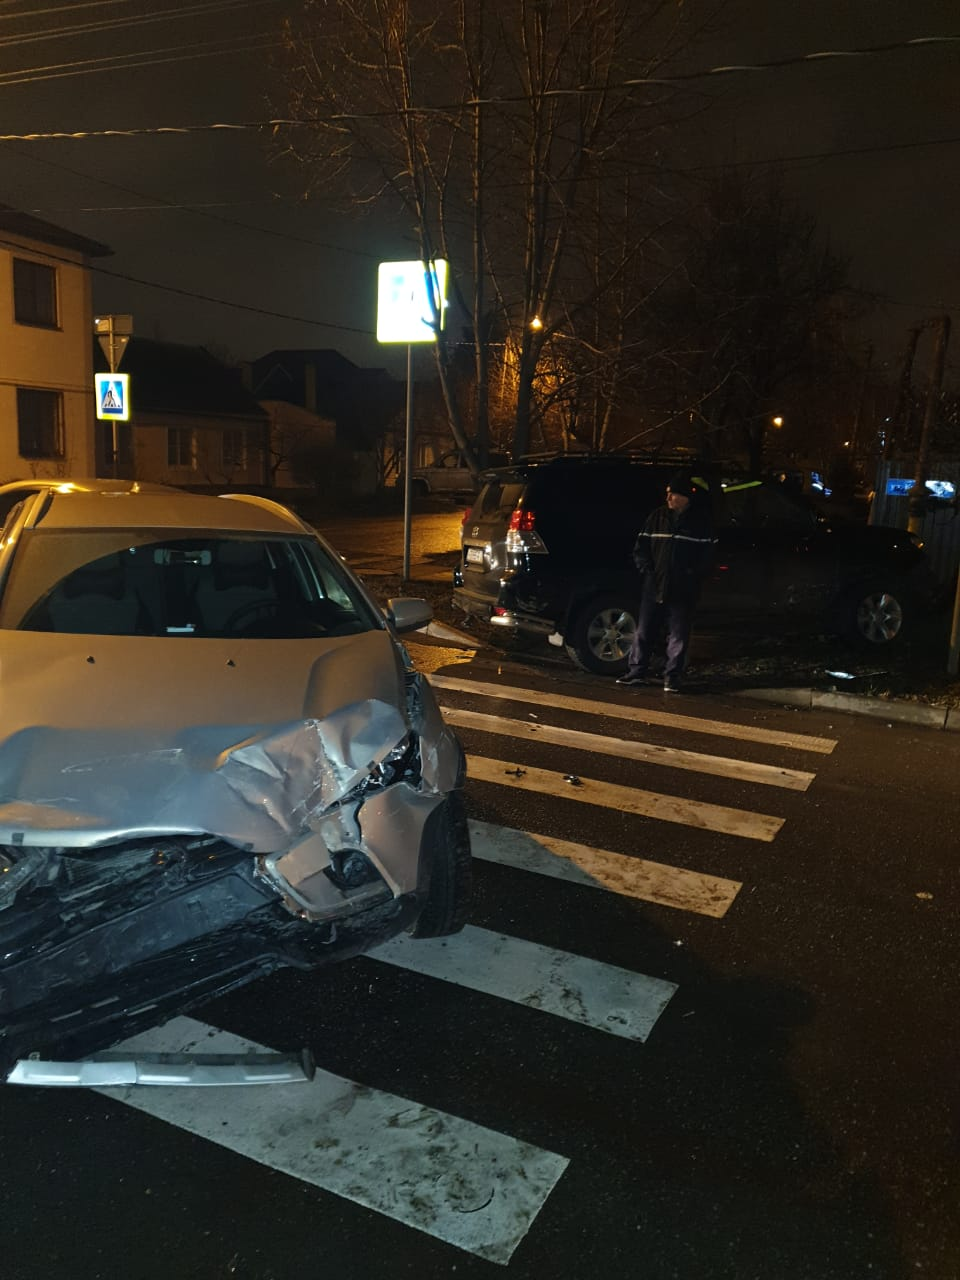
\includegraphics[width=.49\textwidth]{foto/дтп1}
            \caption{\footnotesize {Фото места ДТП. На переднем плане автомобиль второго участника ДТП}}
            \label{ris:images/дтп1}}
        \hfil \hfil%раздвигаем боксы по горизонтали 
        \parbox[t]{0.49\textwidth}
        {\centering
            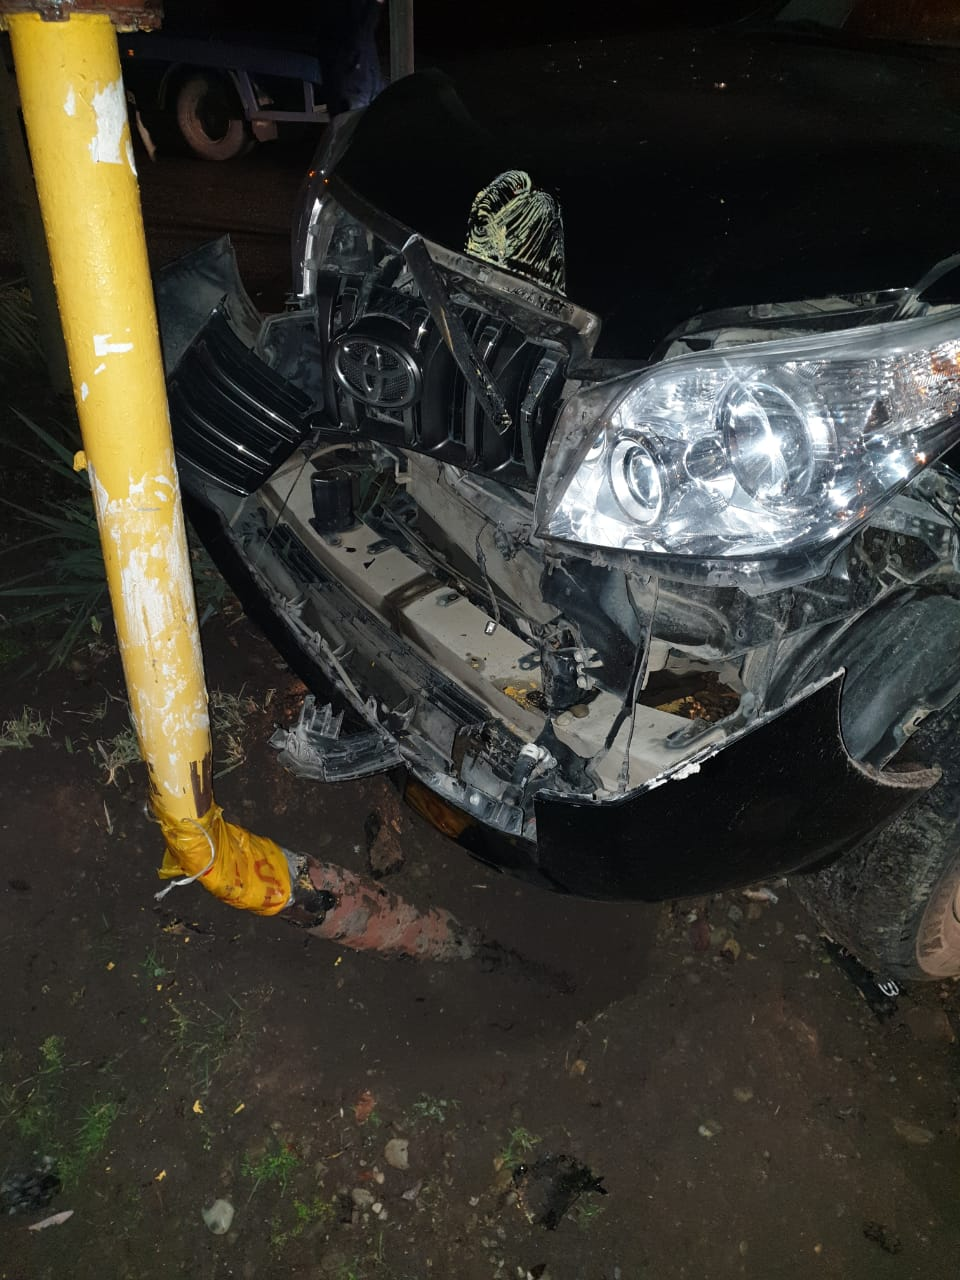
\includegraphics[width=.49\textwidth]{foto/дтп2}
            \caption{\footnotesize {Фото места ДТП. Автомобиль \тс}}
            \label{ris:images/дтп2}}
    \end{figure}
    
    Причины возникновения технических повреждений и возможность их отнесения к
рассматриваемому ДТП исследованы при осмотре ТС. Для определения причины возникновения повреждений, указанных в Акте осмотра ТС  №  \NomerDoc\, (Приложение № 1) экспертом-техником изучены документы, представленные Заказчиком. По предоставленным документам экспертом установлена причина ДТП, установлены обстоятельства ДТП, выявлены повреждения ТС и установлены причины их образования. Проведено исследование характера выявленных повреждений, сопоставление повреждений ТС потерпевшего с повреждениями ТС иных участников ДТП в соответствии со сведениями, зафиксированными в документах о ДТП.  Проведена проверка взаимосвязанности повреждений на ТС с заявленными обстоятельствами ДТП. 

В результате проведённых исследований эксперт-техник приходит к заключению о соответствии механических повреждений, имеющихся на \тс\, регистрационный знак \грз\, на момент осмотра заявленным обстоятельствам. 


\subsubsection{Исследование наличия, характера и объёма технических повреждений}

  Наличие, характер и объем технических повреждений транспортного средства \tc\, регистрационный знак \grz, исследованы в присутствии заинтересованных лиц,  зафиксированы в акте осмотра № \NomerDoc\,  (Приложение, <<Акт осмотра>> ),  и фотоматериалах (Приложение, <<Фототаблица>>) по принадлежности. Планируемые (предполагаемые) ремонтные воздействия для восстановления повреждённого  транспортного средства назначены экспертом-техником с учётом особенностей конструкции и рекомендаций изготовителя  транспортного средства, укрупненных показателей трудозатрат по кузовному ремонту и устранению перекосов проёмов и кузова легковых автомобилей иностранных производителей, приложение 3 к приложению к Положению Банка России от 19 сентября 2014 года № 432-П и приведены ниже в таблице \ref{tab:5}.
 
  %\pagebreak
  
  \begin{longtable}{G{3mm}|M{120mm}|G{30mm}}
      \caption[]{\footnotesize {Повреждения автомобиля, установленные при его осмотре}} 
      \label{tab:5}\\ 
      \hline 
      \hline  \toprule 
\bf  {\footnotesize  n/n}  &\bf {\small Наименование  детали с описанием повреждения} & \bf {\small Изображение} \\   \hline\hline  \toprule \endhead 
%%%%___________________________________________________________________    
\пов{Дверь передняя левая - повреждение лицевой панели средней степени сложности, \s{0.35}}{40}
%%%_____________________________________________________
\пов{Каркас двери передней левой - залом в средней части, \s{0.02}}{42}

\пов{Дверь задняя левая - поврждение панели задней левой двери, \s{0.35}, сложная деформация в передней нижней части, \s{0.05}, повреждение ЛКП и деформация средней степени сложности, \s{0.3}}{9}

\пов{Порог левой боковины - деформация средней степени сложности, \s{0.05}}{11}

\пов{Ручка двери передней левой - счес материала детали}{3}

\пов{Корпус зеркала левого наружного - скол фрагмента детали}{7}
      
  \end{longtable}\setcounter{rownum}{0}
  
  
\subsubsection{Определение стоимости восстановительных расходов}

 В соответствии с существующей экспертной методикой размер расходов на восстановительный ремонт определяется исходя из стоимости ремонтных работ (работ по восстановлению, в том числе окраске, контролю, диагностике и регулировке, сопутствующих работ), стоимости используемых в процессе восстановления транспортного средства деталей (узлов, агрегатов) и материалов взамен повреждённых. Расчёт размера расходов (в рублях) на восстановительный ремонт производится по формуле: 
      
\begin{equation}\label{eq:cr}
C_{\text{вр}}  =\sum{C_{ip}}= \sum\left({T_{ij}}\cdot {C_{i\text{нч}}}\right) + \sum{C_{ip^{\text{\,\,\,руб}}}} , \,\,\,\text{где:} 
\end{equation}
%\vspace{2mm}
\begin{itemize}
	\item[ ]$ C_{ip} $ -- стоимость работ i-го вида: $C_\text {зам} $, $ C_\text{восст} $, $ C_\text{рег} $, $C_\text{контр} $, $ C_\text{антикор} $, $ C_\text{зч} $, $ C_\text{ом} $,$ C_\text{соп} $, $ C_\text{вм} $, руб;
	\item[ ]$ T_{ij} $ -- трудоёмкость j-й операции(комплекса) по i-му виду работ, руб;
	\item[ ]$ C_{i\text{нч}} $ -- стоимость нормо-часа по i-му виду работ, руб;
	\item[ ]$ C_{ip^\text{\,\,руб}} $ -- стоимость работ $ C_{ip} $, принятая непосредственно в денежном выражении, руб.
\end{itemize}

\par При определении стоимости восстановительного ремонта АМТС с учётом износа под износом следует понимать количественную меру физического старения АМТС и его элементов, достигнутого в результате эксплуатации, т.е. эксплуатационный износ.
%
Расчёт износа производится в  соответствии с Положением Банка России от «19» сентября 2014 года № 432-П «О единой методике определения размера расходов на восстановительный ремонт в отношении повреждённого транспортного средства» [3].
Износ комплектующих изделий (деталей, узлов, агрегатов) рассчитывается по следующей формуле:
%
%
%
\begin{equation}\label{eq:I}
\text{И}_{\text{ки}} 
= 100\cdot\left( 1-e^ {-\left( \Delta_{T} \cdot T_{\text{КИ}} + \Delta_{L} \cdot L_{\text{КИ}} \right)}\right), \,\,\,\,\text{где:}   
\end{equation}
%
\begin{itemize}
	\item[ ]$ \text{И}_{\text{ки}} $ -- износ комплектующего изделия (детали, узла, агрегата) (процентов); 
	\item[ ]$ e $ -- основание натуральных логарифмов (e =  2,72);
	\item[ ]$ \Delta_{T}$ --  срок эксплуатации комплектующего изделия (детали, узла, агрегата) (лет);
	\item[ ]$ T_{\text{КИ}} $ -- стоимость работ $ C_{ip} $, принятая непосредственно в денежном выражении, руб;
	\item[ ]$ \Delta_{L} $ -- коэффициент, учитывающий влияние на износ комплектующего (детали, узла, агрегата) величины пробега транспортного средства с этим комплектующим изделием;
	\item[ ]$ L_{\text{КИ}} $ -- пробег транспортного средства на дату дорожно-транспортного происшествия (тысяч километров).  
\end{itemize}
\vspace{5mm}
\par Значения коэффициентов $ \Delta_{T}$  и $ \Delta_{L} $  для различных категорий и марок транспортных средств приведены в п. 5. сп. лит~[3]. При этом, на комплектующие изделия (детали, узлы, агрегаты), которые находятся в заведомо худшем состоянии, чем общее состояние транспортного средства в целом, и его основные части, вследствие влияния факторов, не учтённых при расчёте износа (например, проведение ремонта с нарушением технологии, не устранение значительных повреждений лакокрасочного покрытия), может быть начислен дополнительный индивидуальный износ. 
Износ шины транспортного средства рассчитывается по следующей формуле:
\begin{equation}\label{eq:sh}
\text{И}_{\text{ш}} = \frac{\text{Н}_{\text{н}}-\text{Н}_{\text{ф}}}{\text{Н}_{\text{н}}-\text{Н}_{\text{доп}}} \cdot{100}\%,  \,\,\,\,\text{где:} 
\end{equation}
%
\begin{itemize}
	\item[ ] $ \text{И}_{\text{ш}} $ -- износ шины, \%;
	\item[ ] $ \text{Н}_{\text{н}} $ -- высота рисунка протектора новой шины, мм;
	\item[ ] $\text{Н}_{\text{ф}} $ -- фактическая высота рисунка протектора шины, мм;
	\item[ ] $ \text{Н}_{\text{доп}} $ --минимально допустимая высота рисунка протектора шины в соответствии с требованиями законодательства Российской Федерации, мм.
\end{itemize}
%
\vspace{5mm}
\relax
%\renewcommand\baselinestretch{1}\small\normalsize
%
Износ шины дополнительно увеличивается для шин с возрастом от 3 до 5 лет - на 15 процентов, свыше 5 лет - на 25 процентов.

                                                 
\subsubsection{Данные для расчёта}

\noindent Объект экспертизы:  транспортное средство \tc\,
регистрационный знак \грз;\\ 
VIN: \вин;\\
Пробег:    \пробег км (установлен по показаниям одометра);\\
Год выпуска:     \год;\\ 
Дата ввода в эксплуатацию:  \началоэкспл;\\
Дата ДТП:  \датадтп;\\
Перечень ремонтных воздействий представлен в таблице \ref{tab:6};\\
%Рыночная стоимость ТС: \tc\,
%регистрационный знак \grz \, по данным открытых специализированных информационных источников составляет: $640 000$ (Шестьсот сорок тысяч) рублей.\\
%
%
%    \begin{equation}\label{eq:I}
%    \text{И}_{\text{ки}} 
%    = 100\cdot\left( 1-e^ {-\left( \Delta_{T} \cdot T_{\text{КИ}} + \Delta_{L} \cdot L_{\text{КИ}} \right)}\right), \,\,\,\,\text{где:}   
%    \end{equation}
%   
%  
%\pagebreak
\subsubsection{Ремонтные воздействия, необходимые для устранения повреждений}
\setcounter{rownum}{0}
\begin{longtable}{G{3mm}|M{130mm}|G{5mm}|G{5mm}|G{5mm}}
     \hline %установленные при его осмотре и соответствующие им ремонтные воздействия}}
     %%\label{tab:5}\\
    \hline
    \toprule 
    \bf  {\footnotesize  n/n}  &\bf {\small Наименование  детали и описание повреждения} & \bf {\small E} & \bf {\small I}& \bf {\small L}\\\hline\hline   \toprule  \endhead 
%%%%______________________________________%%%%%%%%%%%%
%%%%%%%%%   ОПИСАНИЕ ПОВРЕЖДЕНИЙ   
%\\ps{ деталь }{E}{I}{L} 
   
\акт{ }{ }{ }{ }
\акт{ }{ }{ }{ }
\акт{ }{ }{ }{ }
%\акт{ }{ }{ }{ }
%\акт{ }{ }{ }{ }
%\акт{ }{ }{ }{ }
%\акт{ }{ }{ }{ }
%\акт{ }{ }{ }{ }
%\акт{ }{ }{ }{ }
%\акт{ }{ }{ }{ }
%\акт{ }{ }{ }{ }
%\акт{ }{ }{ }{ }
%\акт{ }{ }{ }{ }
%\акт{ }{ }{ }{ }
%\акт{ }{ }{ }{ }
%\акт{ }{ }{ }{ }
%\акт{ }{ }{ }{ }

  \end{longtable}\setcounter{rownum}{0} 
%
\subsubsection{ Расчёт}
    
\indent Полный расчёт стоимости восстановительных расходов на ремонт ТС с учётом износа в соответствии с правилами обязательного страхования гражданской ответственности владельцев транспортных средств выполнен в  лицензированном для решения задач в рамках ОСАГО программном комплексе   Audatex ОСАГО Про и приведён в Калькуляции № \NomerDoc.
 Расчёт износа произведён программой  Audatex ОСАГО Про и представлен  в калькуляции расчёта затрат № \NomerDoc.
\indent Результаты расчёта  стоимости восстановительных расходов ТС \тс\, \грз\, представлены ниже:\\
  
  
\begin{figure}[H]
        	\centering
        	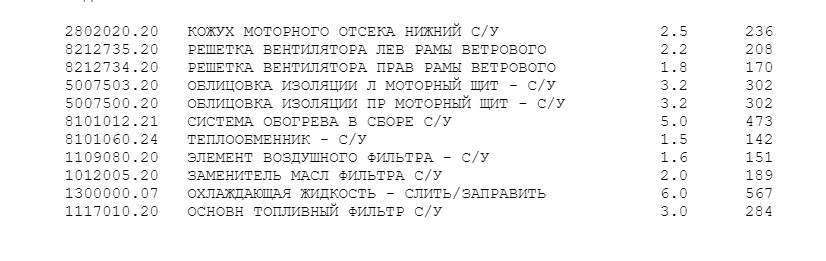
\includegraphics[width=0.95\linewidth]{foto/Screenshot_1}
    %    		\caption{}
    %    		\label{fig:screenshot001}
        \end{figure}
  
    %
    \begin{figure}[H]
    	\centering
    	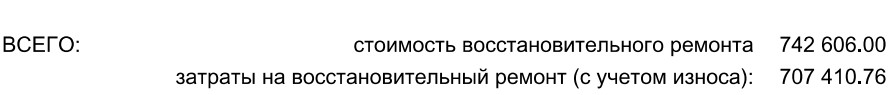
\includegraphics[width=0.95\linewidth]{foto/Screenshot_2}
%    		\caption{}
%    		\label{fig:screenshot001}
    \end{figure}
    \begin{figure}[H]
    	\centering
    	\includegraphics[width=0.95\linewidth]{foto/Screenshot_3}
%    		\caption{}
%    		\label{fig:screenshot002}
    \end{figure}
    \medskip
    \renewcommand\baselinestretch{1.2}\small\normalsize
    

\subparagraph{}Стоимость одного нормо-часа работ определена в соответствии с пунктом 3.8.1 Единой методики [3] путём применения электронных баз данных стоимостной информации.
Трудоёмкость работ по разборке/сборке/замене  соответствует трудоёмкостям работ, рекомендованным заводом изготовителем ТС. Трудоёмкости окрасочных работ приняты согласно рекомендаций Единой методики, п.3.7.1. в соответствии с технологией  AZT (\url{http://www.schwacke.ru/down/azt _reparaturlackierung_ru.pdf}). Расчёт размера расходов на материалы произведён  согласно пункту 3.7.2 Приложения к Единой методике [3]. Артикулы запасных частей определены с помощью программы Audatex и электронных  каталогов запасных частей \url{emex.ru}, \url{partsouq.com}.
Стоимость запасных частей определена в соответствии с пунктом 3.6.3 Единой методики путём применения электронных баз данных стоимостной информации (по утверждённому справочнику: \url{http://prices.autoins.ru/priceAutoParts/repair_parts.html} ).
  
\subparagraph{}Таким образом,  наиболее вероятная стоимость ремонта транспортного средства \tc\, регистрационный знак \грз, получившего повреждения в результате дорожно-транспортного происшествия  \датадтп\, составляет $81 556$ (Восемьдесят одна тысяча пятьсот пятьдесят шесть) рублей,  размер затрат на восстановительный ремонт ТС с учётом износа составляет  $ 52 916 $ (Пятьдесят две тысячи девятьсот шестнадцать) рублей, или с учётом округления составляет $ 53 000 $ (Пятьдесят три тысячи) рублей.
      
% \subsection{Расчет рыночной стоимости ТС}


\par \indent Рыночная стоимость транспортного средства - наиболее вероятная стоимость, по которой транспортное средство может быть отчуждено на открытом рынке в условиях конкуренции, когда стороны сделки действуют разумно, располагая всей необходимой информацией, а на величине стоимости сделки не отражаются какие-либо чрезвычайные обстоятельства [4]. Рыночная стоимость транспортного средства  рассчитывается  для условий конкретных товарных рынков транспортных средств, соответствующих месту государственной регистрации транспортного средства потерпевшего.
\par Определение рыночной стоимости ТС может производится сравнительным и затратным подходом, а именно:  сравнительный анализ продаж (анализ информации о первичном и вторичном рынке АМТС в Российской Федерации);  затратный (с учетом износа АМТС).
\par В оценочной практике наиболее распространенным и предпочтительным является метод прямого сравнения продаж, в соответствии с которым стоимость объекта оценки определяется как средняя цена отобранных аналогов с последующими параметрическими и износными корректировками.   В цены аналогов не вносятся корректировки, если аналоги являются идентичными и равновозрастными объектами по отношению к объекту оценки. 
\par Общий алгоритм метода прямого сравнения продаж:
\begin{list}{-}{}
	\item сбор необходимой информации об объектах;
	\item  производится выборка цен на объекты;
\item  проверка полученной выборки на однородность путем расчета коэффициента вариации;
\item  при значении коэффициента вариации, не превышающем 20\%, определяется средняя цена, которая принимается за стоимость объекта [9]
\item  при превышении коэффициента вариации значения  20\%  выборка исследуется на наличие выбросов с использованием метода Граббса [9,10].
\end{list}
Рыночная стоимость ТС отражает его комплектацию, комплектность, фактическое техническое состояние, срок эксплуатации, пробег, условия, в которых оно эксплуатировалось, коньюктуру первичного и вторичного рынка ТС в регионе. В общем случае расчет рыночной стоимости производится по формуле:
\begin{equation}\label{eq:aa}
C_{\text{КТС}} = C_{cp}\left(1 \pm  \left( \frac{\text{П}_{\text{П}}}{100}\right) \pm\left( \frac{\text{П}_{\text{Э}}}{100}\right) \right) + C_{\text{ДОП}}, \text{руб}
\end{equation}

\noindent где: $C_\text{ср}$ -- средняя цена ТС, \text{руб};\\
$ \text{П}_\text{П}$ -- процентный показатель корректировки средней цены ТС по пробегу, \%;\\
$ C_\text{ДОП}$ -- дополнительное увеличение (уменьшение) стоимости в зависимости от его комплектации, наличия повреждений и акта их устранения, обновления составных частей, руб.\\
Корректировка средней цены ТС, исходя из его комплектности, опций комплектации, обновления составных частей, повреждений и акта их устранения определяется по формуле:
\begin{equation}\label{eq:b}
  C_\text{ДОП}=C_1\pm C_2\pm\left( C_P+C_M+C_\text{ЗЧ}\cdot\left( 1-\text{И}\right) +C_\text{УТС}\right), \text{руб}  
\end{equation} 
где:\\
$C_1$ --увеличение средней цены транспортного средства вследствие замены (обновления его частей в процессе эксплуатации, руб;\\
$ C_2$ -- изменение средней цены транспортного средства в зависимости опций его комплектации, руб;\\
 $ C_P $ -- стоимость ремонтных работ, руб;\\
 $C_M$--  стоимость материалов, руб;\\
 $C_\text{ЗЧ}  $ -- стоимость запасных частей, руб;\\
 $ C_\text{УТС} $ -- величина УТС, руб;\\
 $ \text{И} $ -- величина износа, \%;\\
 
Приоритетным способом определения рыночной стоимость TC
является метод сравнительного подхода, основанный на объективных справочных данных о ценах на подержанные автомобили  в регионе, где проводится оценка.
   
При определении стоимости транспортного средства сравнительным подходом экспертом были использованы  Интернет-источники сведений об аналогах (таблица \ref{tab:5}), содержащие краткое описание основных характеристик и технического состояния. 
 
\begin{longtable}{|p{5mm}|p{85mm}|c|p{60mm}|l|}
	\caption[]{\footnotesize {Описание ТС, идентичных оцениваему}} \label{tab:5}\\ 
	\hline
	%\rowcolor[HTML]{C0C0C0} 
	\rowcolor[HTML]{EFEFEF}
\bf	\text{n/n} &\bf  Описание аналога & \bf URL-адрес преложения  \\ \hline \endhead
		\toprule \centering
\Rownum  &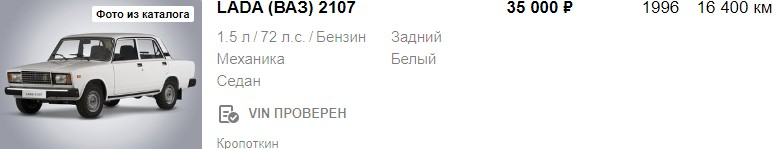
\includegraphics[width=0.99\linewidth]{A_1} &{\noindent \scriptsize\ \url {https://auto.ru/krasnodar/cars/vaz/2107/1996-year/all}} \\ \hline 	\centering
%	\rowcolor[HTML]{EFEFEF} 
\Rownum  &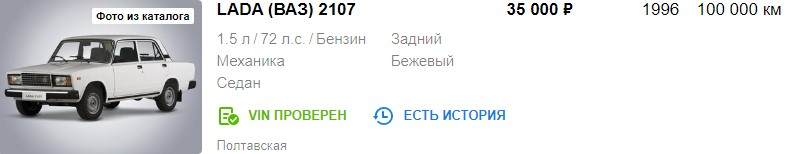
\includegraphics[width=0.99\linewidth]{A_2} & {\noindent \scriptsize\ \url {https://auto.ru/krasnodar/cars/vaz/2107/1996-year/all}} \\ \hline 	\centering
\Rownum  &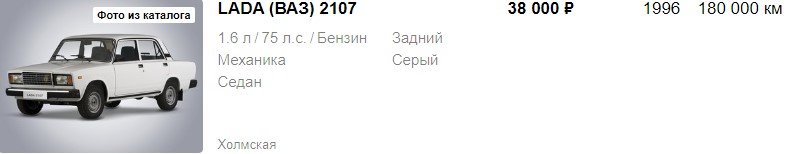
\includegraphics[width=0.99\linewidth]{A_3} &{\noindent \scriptsize\ \url {https://auto.ru/krasnodar/cars/vaz/2107/1996-year/all}} \\ \hline 	\centering
\Rownum  &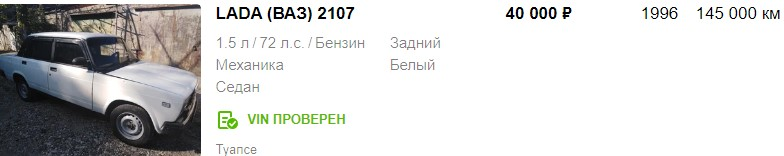
\includegraphics[width=0.99\linewidth]{A_4} &{\noindent \scriptsize\ \url {https://auto.ru/krasnodar/cars/vaz/2107/1996-year/all}} \\ \hline 	\centering
\Rownum &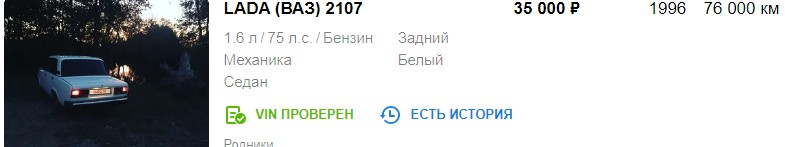
\includegraphics[width=0.99\linewidth]{A_5} &{\noindent \scriptsize\ \url {https://auto.ru/krasnodar/cars/vaz/2107/1996-year/all}} \\ \hline 	\centering
\Rownum  &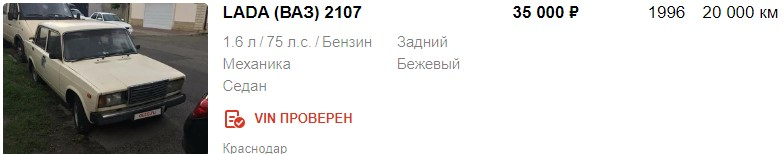
\includegraphics[width=0.99\linewidth]{A_6} &{\noindent \scriptsize\ \url {https://auto.ru/krasnodar/cars/vaz/2107/1996-year/all}}\\ \hline 	\centering
\Rownum  &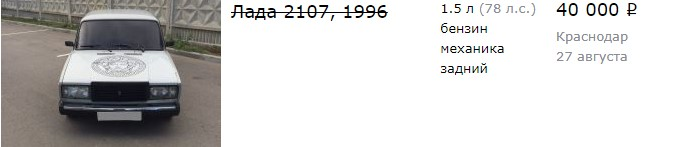
\includegraphics[width=0.99\linewidth]{A_7} &{\noindent \scriptsize\ \url {https://krasnodar.drom.ru/data/2107/35131847}} \\ \hline 	\centering
%\Rownum  &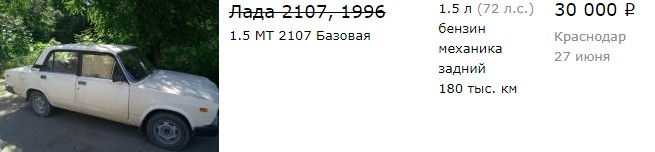
\includegraphics[width=0.99\linewidth]{A_8} &{\noindent \scriptsize\ \url {https://https://krasnodar.drom.ru/lada/2107/34429407}} \\ \hline 	\centering \textbf{}
\Rownum &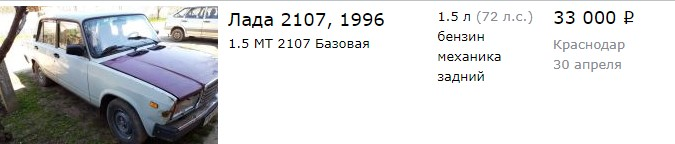
\includegraphics[width=0.99\linewidth]{A_9} &{\noindent \scriptsize\ 
\url {https://krasnodar.drom.ru/lada/2107/33456928}} \\ \hline
					
\end{longtable}
%}

%	1. Определяется \overline{X} – среднее значение цены в %промежуточной выборке по формуле:        
 %
%где n – объем выборки (количество элементов в выборке);
%X_i – цена\  i– го объекта-аналога в промежуточной выборке.
%
%	2. Проверяется полученная выборка на однородность путем расчета %коэффициента вариации. Степень однородности выборки оценивается по %коэффициенту вариации (VB ), измеряющему  рассеивание данных %относительно среднего значения:
%V_B=\frac{\sigma_1}{\overline{X}}100%,  
%где \sigma_1- среднеквадратическое (или стандартное) отклонение, %определяемое по формуле:
%\sigma_1=\sqrt{\frac{\sum_{i=1}^{n}{{(X}_i-\overline{X})}^2}{n-1}};
%D= \frac{\sum_{i=1}^{n}{{(X}_i-\overline{X})}^2}{n-1}, где D -%дисперсия выборки.
	%Для малой выборки принято считать, что если VB <15%, то %однородность выборки высокая; 15% <VB<<25%, однородность выборки %средняя,  25% < VB< 33% однородность выборки низкая [9].
	%4. .При значении коэффициента вариации, не превышающем 20%, %определяется средняя цена, которая принимается за стоимость объекта.
	%5.  При превышении коэффициента вариации значения  20%  выборка %исследуется на наличие выбросов с использованием метода Граббса.
	%Окончательно, рассчитанная средняя цена предложения корректируется %с учетом торга в зависимости  от активности рынка – чем выше %спрос/предложение, тем ниже корректировка на торг. Для данного ТС %наиболее вероятное значение корректировки – 10.9% (данные %аналитического агентства «Автостат» %%http://www.autostat.ru/news/20083/)











%%%%%%%%%% среднеквадратичное отклонение и дисперсия выборки
%где $ \sigma_1 $- среднеквадратическое (или стандартное) отклонение, определяемое по формуле:
%\begin{equation}\label{ab}
%\sigma_1=\sqrt{\frac{\sum\limits_{i=1}^{n}{{(X}_i-\overline{X})}^2}{n-1}}
%\end{equation}
%
%\begin{equation}\label{ac}
%D= \frac{\sum\limits_{i=1}^{n}{{(X}_i-\overline{X})}^2}{n-1}
%\end{equation},
%
%
%где $ D $ -дисперсия выборки.
%Для малой Для малой выборки принято считать, что если VB <15\%, то однородность выборки высокая; 15\% <$  V_B  $<<25\%, однородность выборки средняя,  25\% < VB< 33\% однородность выборки низкая 
%
%4. .При значении коэффициента вариации, не превышающем 20\%, определяется средняя цена, которая принимается за стоимость объекта.
%5.  При превышении коэффициента вариации значения  20\%  выборка исследуется на наличие выбросов с использованием метода Граббса.
%6.	Окончательно, рассчитанная средняя цена предложения корректируется с учетом торга в зависимости  от активности рынка – чем выше спрос/предложение, тем ниже корректировка на торг. Для данного ТС наиболее вероятное значение корректировки – 10.9\% (данные аналитического агентства «Автостат» http://www.autostat.ru/news/20083/)
%
%\par Рыночная стоимость ТС  учитывает его фактическое техническое состояние, условия, в которых оно эксплуатировалось.
% Ремонт кузовных составляющих транспортного средства является фактором, влияющим на уменьшение средней цены ТС. В соответствии с Методикой [1], Приложение 3.3 <<Процентный показатель корректирования средней цены КТС в зависимости от условий эксплуатации>>, Таблица 1, для автомобилей со сроком эксплуатации до 7 лет, при восстановлении трех и больше кузовных составных частей уменьшение рыночной стоимости составляет 10 \%. 

%\par При определении стоимости транспортного средства сравнительным подходом экспертом использованы  Интернет-источники сведений об аналогах (Таблица \ref{tab:5}), содержащие краткое описание основных характеристик и технического состояния. Поскольку при определении рыночной стоимости  эксперту-технику данные о техническом состоянии и условиях эксплуатации не заданы и объективно не могут быть  получены при осмотре ТС на момент исследования, то для расчета принимается следующее:
%\begin{list}{-}{}
%	\item техническое состояние ТС соответствует сроку эксплуатации;
%	\item тс не эксплуатировалось в режиме такси или специальных условий эксплуатации;
%	\item фактический пробег ТС на момент повреждения составлял 45 513 км;
%	\item  29.06.2018 г. ТС \тс \, участвовал в ДТП, в результате которого  автомобиль получил механические повреждения задней правой двери, заднего правого порога, заднего правого колеса,  подушки SRS справа.
%\end{list}

%Из открытых банков данных полиции следует, что автомобиль с VIN: \,  \вин\,  как минимум дважды становился участником ДТП.
%Первый раз 29.06.2018  06:40, извещение о ДТП № 030046913, в котором автомобиль получил повреждения задней правой двери, заднего правого порога, заднего правого колеса, подушки SRS справа, Рис. \ref{ris:images/d1} и второй раз 22.05.2019 06:50, извещение о ДТП № 030034947, в котором автомобиль получил повреждения деталей передней левой и задней частей кузова, Рис. \ref{ris:images/d2}.
%%
%\vspace{\baselineskip}
%%
%\begin{figure}[H]\centering
%	\parbox[t]{0.49\textwidth}
%	{\centering
%		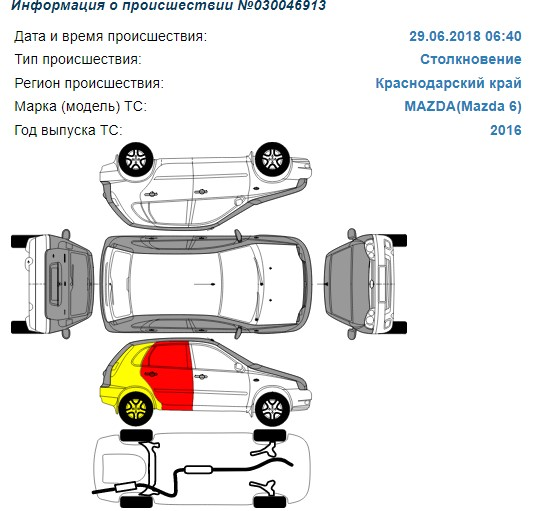
\includegraphics[width=.49\textwidth]{images/d1}
%		\caption{\footnotesize {Повреждения в ДТП 29.06.2018 }}
%		\label{ris:images/d1}}
%	\hfil \hfil%раздвигаем боксы по горизонтали 
%	\parbox[t]{0.49\textwidth}
%	{\centering
%		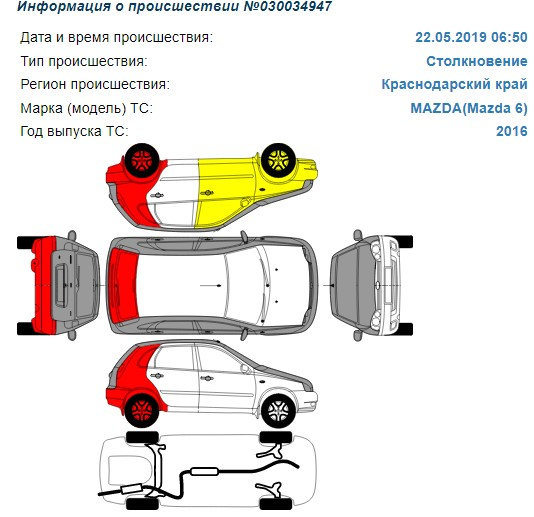
\includegraphics[width=.49\textwidth]{images/d2}
%		\caption{\footnotesize {Повреждения в ДТП 22.05.2019}}
%		\label{ris:images/d2}}
%\end{figure}
%%
%\vspace{\baselineskip}
%
%{\noindent  \footnotesize \tikz \fill [red] (1,0.5) rectangle (0.1,0.1); --{\footnotesize  Вмятины, вырывы, заломы, перекосы, разрывы и другие повреждения с изменением геометрии элементов (деталей) кузова и эксплуатационных характеристик ТС.}\\
%	\tikz \fill [yellow] (1,0.5) rectangle (0.1,0.1); --  {\footnotesize Повреждения колёс (шин), элементов ходовой части, стекол, фар, указателей поворота, стоп-сигналов и других стеклянных элементов (в т.ч. зеркал), а также царапины, сколы, потертости лакокрасочного покрытия или пластиковых конструктивных деталей и другие повреждения без изменения геометрии элементов (деталей) кузова и эксплуатационных характеристик ТС.}\\[1mm]
%	
%\renewcommand\baselinestretch{1.2}\small\normalsize

%\par Вследствие вышеизложенного коэффициент $ C_\text{ДОП}$ принимается равным -10 \%, коэффициенты $ \text{П}_{\text{Э}} $ и $ \text{П}_{\text{П}} $ принимаем равными нулю.

Средняя цена  $C_\text{ср}$  определяется на базе  средней рыночной цены продажи совокупности идентичных ТС на дату оценки: 
\begin{equation}\label{C}
C_\text{ср} =   \frac{ \sum\limits_{i=1}^n{C_i}}{n}
\end{equation}
 $C_\text{ср} =(\sum\limits_{i=1}^n{C_i})/n= (35000+35000+38000+40000+35000+35000+40000+33000)/8 =36 375 $, руб.\\
\noindent где: $ C_i $ - цена предложения к продаже i-го ТС, \\
\indent i - количество предложений, i=8.
\par Поскольку используемая выборка состоит из цен предложений к продаже, то для приведения к средней рыночной цене покупки применяется коэффициент торга $ K_T $, значение которого согласно данных аналитического агентства «Автостат» http://www.autostat.ru/news/20083/, %рис. \ref{fig:avtostat} 
\, составляет 5 \%. Соответственно, средняя цена предложений должна быть скорректирована в соответствии с нижеприведенной формулой \ref{Cp}:
\begin{equation}\label{Cp}
C_\text{ср} =  \left( \sum\limits_{i=1}^n{C_i}\right)  \cdot K_T , \,\, \text{руб}
\end{equation}
%%%%%%%%%%%%%%%%%%%%%  График АВТОСТАТ (если нужно)
%\begin{figure}
%	\centering
%	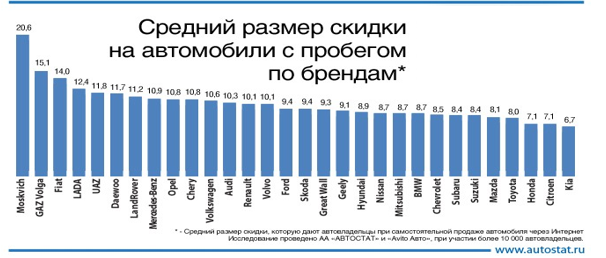
\includegraphics[width=0.7\linewidth]{images/avtostat}
%	\caption{График аналитического агентства <<Автостат>> процента уторговывания по маркам автомобилей}
%	\label{fig:avtostat}
%\end{figure}
Тогда,\,\, рыночная стоимость $ C $ автомобиля \тс \, с учетом торга и факторов, влияющих на рыночную стоимость составляет: 
\begin{equation}\label{cp}
C = C_\text{ср} \cdot  K_T 
%-  C_\text{ДОП} 
= 36375 \cdot(100-5)
%)\cdot 0.9 
=  34556 \, \, \text{руб},
\end{equation} 
\noindent что с учетом округления составляет 35000  рублей.

\par Таким образом, рыночная стоимость ТС \тс, \, с учетом всех имеющихся сведений о состоянии ТС на момент повреждения \датадтп\,  составляет 35000 (Тридцать пять тысяч) рублей.

%\paragraph*{} Федеральным законом от 25.04.2002 года № 40-ФЗ «Об обязательном страховании гражданской ответственности владельцев транспортных средств» в редакции на момент заключения договоров страхования и страхового случая (далее – Закон об ОСАГО) установлено:
%(пункт 18 статьи 12) что размер подлежащих возмещению страховщиком убытков при причинении вреда имуществу потерпевшего определяется: \par а) в случае полной гибели имущества потерпевшего - в размере действительной стоимости имущества на день наступления страхового случая за вычетом стоимости годных остатков. Под полной гибелью понимаются случаи, при которых ремонт поврежденного имущества невозможен либо стоимость ремонта поврежденного имущества равна стоимости имущества на дату наступления страхового случая или превышает указанную стоимость.\par Настоящим исследованием установлено, что стоимость восстановительного ремонта ТС \тс \, превышает рыночную стоимость ТС на момент повреждения. Таким образом, при определении стоимости восстановительных расходов необходимо произвести расчет стоимости годных остатков ТС.
%\par  
%Положением Банка России от 19 сентября 2014 г. N 432-П "О единой методике определения размера расходов на восстановительный ремонт в отношении поврежденного транспортного средства <<Глава 5. Порядок расчета стоимости годных остатков в случае полной гибели транспортного средства>> установлен алгоритм расчета годных остатков ТС.




%\subsection{Расчёт утраты товарной стоимости ТС}

\par В целях обеспечения единства практики применения судами законодательства, регулирующего отношения в области обязательного страхования гражданской ответственности владельцев транспортных средств, Пленум Верховного Суда Российской Федерации, руководствуясь статьей 126 Конституции Российской Федерации, статьями 2 и 5 Федерального конституционного закона от 5 февраля 2014 года N 3-ФКЗ "О Верховном Суде Российской Федерации", постановляет дать следующие разъяснениz
Общие положения Постановление Пленума Верховного Суда Российской Федерации от 26 декабря 2017 г. N 58 г. Москва "О применении судами законодательства об обязательном страховании гражданской ответственности владельцев транспортных средств" 

п. 37. К реальному ущербу, возникшему в результате дорожно-транспортного происшествия, наряду со стоимостью ремонта и запасных частей относится также утрата товарной стоимости, которая представляет собой уменьшение стоимости транспортного средства, вызванное преждевременным ухудшением товарного (внешнего) вида транспортного средства и его эксплуатационных качеств в результате снижения прочности и долговечности отдельных деталей, узлов и агрегатов, соединений и защитных покрытий вследствие дорожно-транспортного происшествия и последующего ремонта.

 Утрата товарной стоимости подлежит возмещению и в случае, если страховое возмещение осуществляется в рамках договора обязательного страхования в форме организации и (или) оплаты восстановительного ремонта повреждённого транспортного средства на станции технического обслуживания, с которой у страховщика заключён договор о ремонте транспортного средства, в установленном законом пределе страховой суммы.

\par Расчёт утраты товарной стоимости в настоящем исследовании производится согласно \emph {Методическим рекомендациям по проведению судебных автотехнических экспертиз и исследований колёсных транспортных средств в целях определения размера ущерба, стоимости восстановительного ремонта и оценки}  [6].

\par Утрата товарной стоимости (УТС) обусловлена снижением товарной стоимости из-за ухудшения потребительских свойств вследствие наличия дефектов (повреждений), или следов их устранения либо наличия достоверной информации, что дефекты (повреждения) устранялись [6, п. 8].

	УТС может быть рассчитана для ТС, находящихся как в повреждённом, так и в отремонтированном состоянии (при возможности установить степень повреждения).

УТС может определяться при необходимости выполнения одного из нижеперечисленных видов ремонтных воздействий или если установлено их выполнение:

-	устранение перекоса кузова или рамы ТС;

-	замена несъемных элементов кузова ТС (полная или частичная); ремонт съёмных или несъемных элементов кузова (включая оперение) ТС (в том числе пластиковых капота, крыльев, дверей, крышки багажника);

-	полная или частичная окраска наружных (лицевых) поверхностей кузова (включая оперение) ТС, бамперов;

-	полная или частичная разборка салона ТС, вызывающая нарушение качества заводской сборки.

УТС не рассчитывается:

а)	если срок эксплуатации легковых автомобилей превышает 5 лет;

б)	если легковые автомобили эксплуатируются в интенсивном режиме, а срок эксплуатации превышает 2,5 года;


в)	в случае замены кузова до оцениваемых повреждений (за исключением кузова грузового КТС, установленного на раме за кабиной);

%)	если КТС ранее подвергалось восстановительному ремонту (в том числе окраске - полной, наружной, частичной; «пятном с переходом») или имело аварийные повреждения, кроме повреждений, указанных в [6, п. 8.4];

д)	если КТС имело коррозионные повреждения кузова или кабины на момент происшествия.



Нижеприведенные повреждения не требуют расчёта УТС вследствие исследуемого происшествия, а их наличие до исследуемого происшествия не обуславливает отказ от расчёта УТС при таких повреждениях:

а)	эксплуатационных повреждениях ЛКП в виде меления, трещин, а также повреждений, вызванных механическими воздействиями - незначительных по площади сколов, рисок, не нарушающих защитных функций ЛКП составных частей оперения;

б)	одиночного эксплуатационного повреждения оперения кузова (кабины) в виде простой деформации, не требующего окраски, площадью не более 0,25 дм2;

в)	повреждения, которые приводят к замене отдельных составных частей, которые не нуждаются в окрашивании и не ухудшают внешний вид КТС (стекло, фары, бампера неокрашиваемые, пневматические шины, колёсные диски, внешняя и внутренняя фурнитура и т. п.). Если, кроме указанных составных частей, повреждены составные части кузова, рамы, кабины или детали оперения - крылья съёмные, капот, двери, крышка багажника, - то расчёт величины УТС должен учитывать все повреждения составных частей в комплексе;

г)	в случае окраски молдингов, облицовок, накладок, ручек, корпусов зеркал и других мелких наружных элементов, колёсных дисков.

В случае исследуемого события для автомобиля \тс\, VIN \vin\,  условия,  при которых производится расчёт УТС выполняются.\\


\par Величина УТС зависит от вида, характера и объёма повреждений и ремонтных воздействий по их устранению.
\par Величина УТС ($ C_\text{YTC} $) определяется на дату оценки (исследования) по формуле: 

\begin{equation}\label{uts}
C_{YTC} = C_{TC} \cdot \dfrac{\sum\limits_{i=1}^n K_{YTCi}}{100\%},\hspace{5mm} \text{руб.},
\end{equation}

\noindent где:\\
\noindent $ C_{TC} $ -- стоимость ТС на дату оценки (исследования), руб;\\
$ K_{YTCi} $ -- коэффициент УТС по i-му элементу КТС, ремонтному воздействию, \%.
 
\par Рыночная стоимость транспортного средства ( $ C_{TC} $ ), согласно п.6.1. Единой методики [3], принимается равной средней стоимости аналога на указанную
дату по данным имеющихся инфор\-мационно-справочных материалов,
содержащих сведения о средней стоимости транспортного средства.

\par  При ремонте съёмной составной части сумма стоимости ремонта (включая стоимость разборки для ремонта и при необходимости снятия детали для ремонта) и величины УТС (без учёта УТС вследствие окраски) не должна превышать суммы стоимости этой составной части (с учётом коэффициента износа) и стоимости работ по ее замене.

\par   Значение коэффициента УТС $ K_{\text{утсокр}} $ при подетальной окраске наружных поверхностей кузова ТС рассчитывается с учётом количества окрашиваемых кузовных составных частей и бамперов по формуле:

\begin{equation}\label{f:yc}
K_{\text{утсокр}}=K_{\text{утсокр(1)}}+K_{\text{утсокр(N-1)}}\cdot(N-1), \hspace{5mm} \% 
\end{equation}
        
\noindent где:\\
\noindent $ \text{К}_{\text{утсокр(1)}} $ - коэффициент УТС по окраске первой кузовной составной части или бампера, \%;\\
$ \text{К}_{\text{утсокр(N-1)}} $ - коэффициент УТС по окраске второй и каждой следующей кузовной составной части или бампера, \%;\\
N - количество окрашиваемых составных частей, по которым рассчитывается УТС.\\
Значения коэффициентов УТС ($ K_{YTC} $) определены по результатам экспертной практики и приведены в приложении [6, Приложение 2.9].

\par Для исследуемого автомобиля \тс \, соответствующие ремонтным воздействиям  коэффициенты УТС приведены ниже в таблице:

\begin{table}[H]
		%\caption{}
	\begin{tabular}{|p{5mm}|p{80mm}|c|c|c|}
	\hline 
	\textbf{п/п} & \textbf{Наименование детали} &\textbf{ К-замена }& \textbf{К-ремонт }&\textbf{ К-окраска} \\ 
	\hline 
	1 & Дверь задняя левая & -- & -- & 0,5 \\ 
	\hline 
%	2 & Бампер задний & -- & -- & 0,35 \\ 
%	\hline 
	2 & Боковина левая & -- & 0,2 & 0,35 \\ 
	\hline 
		3 & Порог левой боковины  & -- & 0,2 & 0,35 \\ 
	\hline 

	
\end{tabular} 

\end{table}

\vspace{7mm}

$  \sum\limits_{i=1}^n K_{YTCi} = 0.5+0.2+0.35+0.2+0.35 = 1.6$\\
  
  
Рыночная стоимость транспортного средства \тс\, на момент повреждения по данным справочника \url { https://automama.ru/krasnodar/cars/ } составляет 660 000 (Шестьсот шестьдесят тысяч) рублей.
  
$   C_{TC} = C_{TC} \cdot \dfrac{\sum\limits_{i=1}^n K_{YTCi}}{100} = 660000 \cdot 1.6/100 = 10560 $%, или с учетом округления 372000 (Триста семьдесят две тысячи) рублей.\\
(Десять тысяч пятьсот шестьдесят) рублей.

\par Таким образом, величина УТС автомобиля \тс\, составляет (Десять тысяч пятьсот шестьдесят) рублей.
%\subsection{Расчёт стоимости годных остатков}



\par \indent  Согласно пп. <<a>> п. 18 ст. 12 Федерального закона  N 40-ФЗ  <<Об обязательном страховании гражданской ответственности владельцев транспортных средств>>  в случаях, при которых ремонт повреждённого имущества невозможен либо стоимость ремонта равна стоимости имущества на дату наступления страхового случая или превышает указанную стоимость размер подлежащих возмещению страховщиком убытков при причинении вреда имуществу потерпевшего определяется в размере действительной стоимости имущества на день наступления страхового случая за вычетом стоимости годных остатков. 

В нашем случае,  стоимость ремонта ТС \тс\, регистрационный знак \грз\, превышает его рыночную стоимость. Следовательно, в порядке, предусмотренном  Главой 5 Положения Банка России от 19 сентября 2014 г. № 432-П <<О единой методике определения размера расходов на восстановительный ремонт в отношении повреждённого транспортного средства>>  производится расчёт стоимости годных остатков. 

\par Под годными остатками автотранспортного средства понимаются работоспособные, имеющие остаточную стоимость детали (агрегаты, узлы) повреждённого автотранспортного средства, как правило, годные к дальнейшей эксплуатации, которые можно демонтировать с повреждённого автотранспортного средства и реализовать. 
Годные остатки должны отвечать следующим условиям:

1) деталь (агрегат, узел) не должна иметь повреждений, нарушающих ее целостность и товарный вид, а агрегат (узел), кроме того, должен находиться в работоспособном состоянии;

2) деталь (агрегат, узел) не должна иметь изменений конструкции, формы, целостности и геометрии, не предусмотренных изготовителем автотранспортного средства (например, дополнительные отверстия и вырезы для крепления несерийного оборудования);

3) деталь не должна иметь следов предыдущих ремонтных воздействий (следов правки, рихтовки, следов шпатлевки, следов частичного ремонта и т.д.).



 Стоимость годных остатков с учётом затрат на их демонтаж, дефектовку, хранение и продажу определяется по формуле:
 \begin{equation}\label{go}
C_{\text{ГО}}= C_{\text{Р}} \cdot K_{\text{В}}\cdot K_{\text{З}}\cdot K_{\text{ОП}} \cdot  \sum\limits_{i-1}^{n}\frac{C_i}{100}, \, \, \text{руб} 
\end{equation}
\noindent где: \,$ C_{\text{Р}} $ -- стоимость ТС в неповрежденном виде на момент происшествия;\\
$ K_{\text{З}} $-- коэффициент, учитывающий затраты на дефектовку, разборку, хранение, продажу;\\
$ K_{\text{В}} $ -- коэффициент, учитывающий срок эксплуатации АМТС на момент повреждения и спрос на его неповреждённые детали;\\
$ K_{\text{ОП}} $ -- коэффициент, учитывающий объем (степень) механических повреждений автомобиля;\\
$ C_i $ процентное соотношение (вес) стоимости неповреждённых элементов к стоимости автомобиля;\\
$ n  $- количество неповреждённых элементов (агрегатов, узлов).\\

Расчёт процентного соотношения (веса) стоимости неповреждённых элементов к стоимости ТС   \,\,
     % \begin{equation}\label{bb}
   $  \left( \sum\limits_{i-1}^{n}\frac{C_i}{100} \right)  $  
%   \end{equation}  
включает только установленные неповреждённые детали, узлы и агрегаты. Компоненты ТС, имеющие повреждения  вероятностного характера, и требующие диагностических работ для установления годности в расчёте не учитываются. 
 
  \begin{longtable}{|p{9cm}|p{4cm}|p{2cm}|}
 	\caption[]{\footnotesize {Таблица расчёта $ C_i $ }}
 	 \label{tab:7}\\
 	 \hline
 	 		Наименование агрегата, узла, детали & \%-ное соотношение (вес)  & Годные, \% \\
 	 		\hline \endhead
 		Кузовные детали, экстерьер, интерьер, в т.ч.: & 50 (45 \textless{}1\textgreater{}) & 0 \\
 		Передняя часть: & 14 &  \\
 		Капот & 1.9 & 1,9 \\
 		Крыло переднее (за 1 шт.) & 0.8 & 0,8 \\
 		Бампер передний (в сборе с усилителем, накладками и молдингами, спойлером) & 1.9 & 1,9 \\
 		Решетка (облицовка) радиатора & 0.8 & 0,8 \\
 		Лонжерон передний (за 1 шт.) & 0.8 & 0,8 \\
 		Брызговик крыла (за 1 шт.) & 1.4 & 1,4 \\
 		Стекло ветрового окна & 1.7 & 1,7 \\
 		Рамка радиатора & 1.4 & 1,4 \\
 		Щиток передка & 0.3 & 0,3 \\
 		Задняя часть: & 12 (14 \textless{}1\textgreater{}) & 0 \\
 		Бампер задний & 1.6 & 0 \\
 		Крыло заднее (боковина \textless{}1\textgreater{}) в сборе с арками (за 1 шт.) & 2.1 (3.1 \textless{}1\textgreater{}) & 0 \\
 		Стекло окна задка & 1.9 & 0 \\
 		Панель задка & 0.8 & 0 \\
 		Пол багажника & 0.8 & 0 \\
 		Облицовки багажника & 1.1 & 0 \\
 		Крышка багажника (дверь задка) & 1.6 & 0 \\
 		Средняя часть: & 24 (17 \textless{}1\textgreater{}) & 0 \\
 		Передняя стойка боковины (за 1 шт.) & 1.4 & 2,8 \\
 		Средняя стойка боковины с порогом и частью пола (за 1 шт.) & 1.4 (0 \textless{}1\textgreater{}) & 2,8 \\
 		Облицовки стоек боковины, порогов, уплотнители, центральная консоль, противосолнечные козырьки, плафоны освещения, коврики пола, зеркало заднего вида & 2.5 (2.1 \textless{}1\textgreater{}) & 2,5 \\
 		Двери в сборе с арматурой (за 1 шт.), & 1.9 & 5,7 \\
 		в т.ч. арматура дверей (за 1    дверной комплект) & 0.5 & 0 \\
 		Сиденья (все) & 1.1 & 1,1 \\
 		Панель крыши в сб. с обивкой, поперечинами и верх. частями стоек, & 3.5 & 2,7 \\
 		в т.ч. обивка панели крыши & 0.8 & 0 \\
 		Панель приборов в сборе с щитком приборов, решётками, вещевым ящиком, карманами и т.д. & 2.5 & 2,5 \\
 		Ремень безопасности передний (за 1 шт.) & 0.3 & 0,6 \\
 		Подушка безопасности пассажирская & 0.6 & 0,6 \\
 		Двигатель, навесное, охлаждение, впускная и выпускная система & 11 (13 \textless{}2\textgreater{}) & 13 \\
 		Двигатель в сборе без навесного оборудования & 4.9 & 0 \\
 		в т.ч. клапанная крышка & 0.5 & 0 \\
 		в т.ч. масляный поддон & 0.5 & 0 \\
 		в т.ч. блок цилиндров & 2.2 & 0 \\
 		Дроссельный узел в сборе с заслонкой, клапаном и датчиком & 1.4 & 0 \\
 		Генератор & 0.8 & 0 \\
 		Коллектор впускной & 0.5 & 0 \\
 		Коллектор выпускной & 0.5 & 0 \\
 		Радиатор охлаждения в сборе с кожухами, вентилятором & 0.8 & 0 \\
 		Стартер & 0.5 & 0 \\
 		Короб воздушного фильтра с патрубками & 0.5 & 0 \\
 		Выпускной тракт в сборе & 0.8 & 0 \\
 		Турбокомпрессор (турбонагнетатель) & 1.4 \textless{}2\textgreater{} & 0 \\
 		Интеркулер & 0.6 \textless{}2\textgreater{} & 0 \\
 		Топливная система & 2.5 & 2,5 \\
 		Бак топливный & 0.7 & 0 \\
 		Система подачи топлива & 1.8 & 0 \\
 		Трансмиссия & 4.5 & 4,5 \\
 		Усреднённый показатель с учётом всех возможных вариантов трансмиссии & 4.5 & 0 \\
 		Подвеска & 10 & 4 \\
 		Подвеска передняя в сборе с поперечиной & 5.5 (4.5 \textless{}4\textgreater{}) & 0 \\
 		Подвеска задняя в сборе с поперечиной & 4.5 (5.5 \textless{}4\textgreater{}) & 4,5 \\
 		Подвеска в сборе для полноприводных АМТС & 10 (5 \textless{}4\textgreater + 5 \textless{}4\textgreater{}) & 0 \\
 		Рулевое управление & 3 & 3 \\
 		Рулевая колонка в сборе с валом & 0.5 & 0 \\
 		Насос ГУР & 0.8 & 0 \\
 		Рулевой механизм & 1.2 & 0 \\
 		Рулевое колесо в сборе с подушкой безопасности & 0.5 & 0 \\
 		в т.ч.: подушка безопасности  водительская & 0.3 & 0 \\
 		Тормозная система & 3.5 & 3,5 \\
 		Главный тормозной цилиндр & 0.5 & 0 \\
 		Тормозной механизм колеса (за каждый колёсный узел) & 0.5 & 0 \\
 		Ручной (ножной) тормоз & 0.3 & 0 \\
 		Блок управления АБС & 0.7 & 0 \\
 		Электрооборудование & 12.5 & 0 \\
 		Провода свечные с катушками (комплект) & 0.5 & 0,5 \\
 		Монтажный блок & 0.5 & 0,5 \\
 		Блок управления двигателем & 1 & 1 \\
 		Фонари задние (за 1 шт.) & 0.5 & 1 \\
 		Зеркала заднего вида боковые (за 1 шт.) & 0.8 & 1,6 \\
 		Блок отопителя салона в сборе (корпус, двигатель, радиаторы) & 2.1 & 2,1 \\
 		Насос кондиционера & 0.5 & 0,5 \\
 		Конденсатор в сборе с осушителем, кожухом, вентилятором, трубками & 0.6 & 0,6 \\
 		Фары (за 1 шт.) & 1.1 & 1,1 \\
 		Жгут проводов ДВС & 0.9 & 0,9 \\
 		Жгут проводов панели приборов & 0.8 & 0,8 \\
 		Остальные жгуты проводов (все) & 0.3 & 0,3 \\
 		Фара противотуманная (за 1 шт.) & 0.8 & 1,6 \\ 
 		Прочее & 3/8 \textless{}1\textgreater{}/1 \textless{}2\textgreater /6 \textless{}3\textgreater{} & 4 \\
 		\hline
 		\textbf{ИТОГО,} \%: &  & \textbf{83,8}  \\
 		\hline	
 	\end{longtable}
 
\noindent  \begin{table}[H]
  	 \label{tab:KB}
	\caption{\footnotesize {Значения коэффициента Кв, учитывающего срок эксплуатации ТС}}
		 \begin{tabular}{|p{47mm} |p{53mm}| p{50mm}|}
	\hline
 		Срок эксплуатации автомобиля, лет & Значение Кв легковых автомобилей, малотоннажных грузовых на базе легковых и мототехники & Значение Кв грузовых автомобилей \\ \hline
 		0 - 5 (включительно)   &0.80                                                                                    & 0.80                             \\ \hline
 		6 - 10 (включительно)             & 0.65                                                                                    & 0.60                             \\ \hline
 		11 - 15 (включительно)            & 0.55                                                                                    & 0.50                             \\ \hline
 		16 - 20 (включительно)            & 0.40                                                                                    & 0.35                             \\ \hline
 		Более 20 лет                      & 0.35                                                                                    & 0.30                            \\ \hline
 	\end{tabular}
\end{table}


\noindent \begin{table}[H]
	\label{tab:KO}
	\caption{\footnotesize {Значение коэффициента $ K_{\text{оп}} $ , учитывающего объем (степень) механических повреждений автомобиля}} 
	\centering
\begin{tabular}{|p{47mm}| p{53mm}| p{50mm}|}
	\hline
	Объем механических повреждений & Соотношение стоимости неповреждённых элементов к стоимости автомобиля, Ci, \% & Значение коэффициента, учитывающего объем механических повреждений \\ \hline
	Незначительный     & 80 -    & 0.9 -  \\
	& 60 - 80      & 0.8 - 0.9      \\
	Средний    & 40 -     & 0.7 -    \\
	& 20 - 40     & 0.6 - 0.7         \\
	Значительный                   & 0 - 20                                                                        & 0.5 - 0.6                                                          \\ \hline
\end{tabular}
\end{table}

 \par
 
% \begin{equation}\label{k}
% C_{\text{ГО}}= C_{\text{Р}} \cdot K_{\text{В}}\cdot K_{\text{З}}\cdot K_{\text{ОП}} \cdot  \sum\limits_{i-1}^{n}\frac{C_i}{100} 
% \end{equation}
 
 Для исследуемого транспортного средства применимы следующие значения коэффициентов:\par
 $ K_{\text{В}} =0.8  $; 
 $ K_{\text{З}} =0.7 $; 
 $ K_{\text{ОП}} =0.8 $; $ \sum\limits_{i-1}^{n}\frac{C_i}{100} = 0.838 $ \par тогда:
 \par
$  C_{\text{ГО}} =  C_{\text{ГО}}= C_{\text{Р}} \cdot K_{\text{В}}\cdot K_{\text{З}}\cdot K_{\text{ОП}} \cdot  \sum\limits_{i-1}^{n}\frac{C_i}{100} =980000*0.8*0.7*0.8*0.838 = 367915 $ руб., или с учётом округления 370 000 (Триста семьдесят тысяч) рублей.
\par Таким образом, стоимость годных остатков ТС \тс \, \, составляет 370 000 (Триста семьдесят тысяч) рублей.



\section{В ы в о д ы}

1) Наличие, характер и объем (степень) технических повреждений, причинённых ТС, определены при осмотре и зафиксированы в Акте осмотра № \NomerDoc\,  фототаблице повреждений и таблице \ref{tab:5}, являющимися неотъемлемой частью настоящего экспертного заключения.\\[3mm]
    
2) Направление, расположение и характер повреждений определены путём сопоставления полученных повреждений, изучения административных материалов по рассматриваемому событию, и  являются  следствиями рассматриваемого ДТП (события).\\[3mm]
    
3) Технология и объем необходимых ремонтных воздействий зафиксированы в калькуляции № \NomerDoc\, по определению стоимости восстановительного ремонта транспортного средства \tc\, VIN  \vin. \\[3mm]
    
4)  Стоимость восстановительного ремонта  транспортного средства \tc\, регистрационный знак \грз,\, \, получившего механические повреждения в результате дорожно-транспортного происшествия, имевшего место \датадтп\, с участием транспортных средств \тс\, регистрационный знак \грз\, и \tca\, составляет $81 556$ (Восемьдесят одна тысяча пятьсот пятьдесят шесть) рублей\\[3mm]
    
5) Размер затрат на проведение восстановительного ремонта с учётом износа (восстановительные расходы) транспортного средства \tc\, регистрационный знак \grz\, составляет  $ 52 916 $ (Пятьдесят две тысячи девятьсот шестнадцать) рублей, или с учётом округления составляет $ 53 000 $ (Пятьдесят три тысячи) рублей.\\[3mm]
    
    
%    6) Стоимость годных остатков ТС \тс\, регистрационный знак \грз\, оставляет  $ 10\,560$ (Десять тысяч пятьсот шестьдесят) рублей.
    
%    6) Величина утраты товарной стоимости транспортного средства \тс\,  регистрационный знак \грз\, составляет  
    
\vspace{10mm}

 \noindent Эксперт-техник   \hfill        Юркова Е.А.
 
\vspace{1mm}
\noindent   \textit{  Государственный  реестровый номер эксперта-техника:   5273}\\

\vspace{15mm}

\relax
\noindent Приложение к заключению:\\
\textit{
%	Приложение № 1. Расшифровка модельных опций ТС \тс \\
    Приложение № 1. Акт осмотра ТС \тс\\
    Приложение № 2. Фототаблица повреждений ТС\\
	Приложение № 3. Калькуляция стоимости восстановительных расходов ТС \тс\\
%	Приложение № 4. Цифровые копии регистрационных документов ТС\\
%	Приложение № 4. Цифровая копия постановления по делу об административном правонарушении дорожно-транспортном происшествии\\
	Приложение № 5. Правоустанавливающие документы эксперта-техника\\
}

%\includepdf[pages=-]{myfile.pdf}
%\includepdf[pages=-]{calc.pdf}